% This is part of Un soupçon de mathématique sans être agressif pour autant
% Copyright (c) 2015
%   Laurent Claessens
% See the file fdl-1.3.txt for copying conditions.

\begin{exercice}\label{exo2smath-0093}

    Anne-Laure a dessiné ce triangle à main levée :
        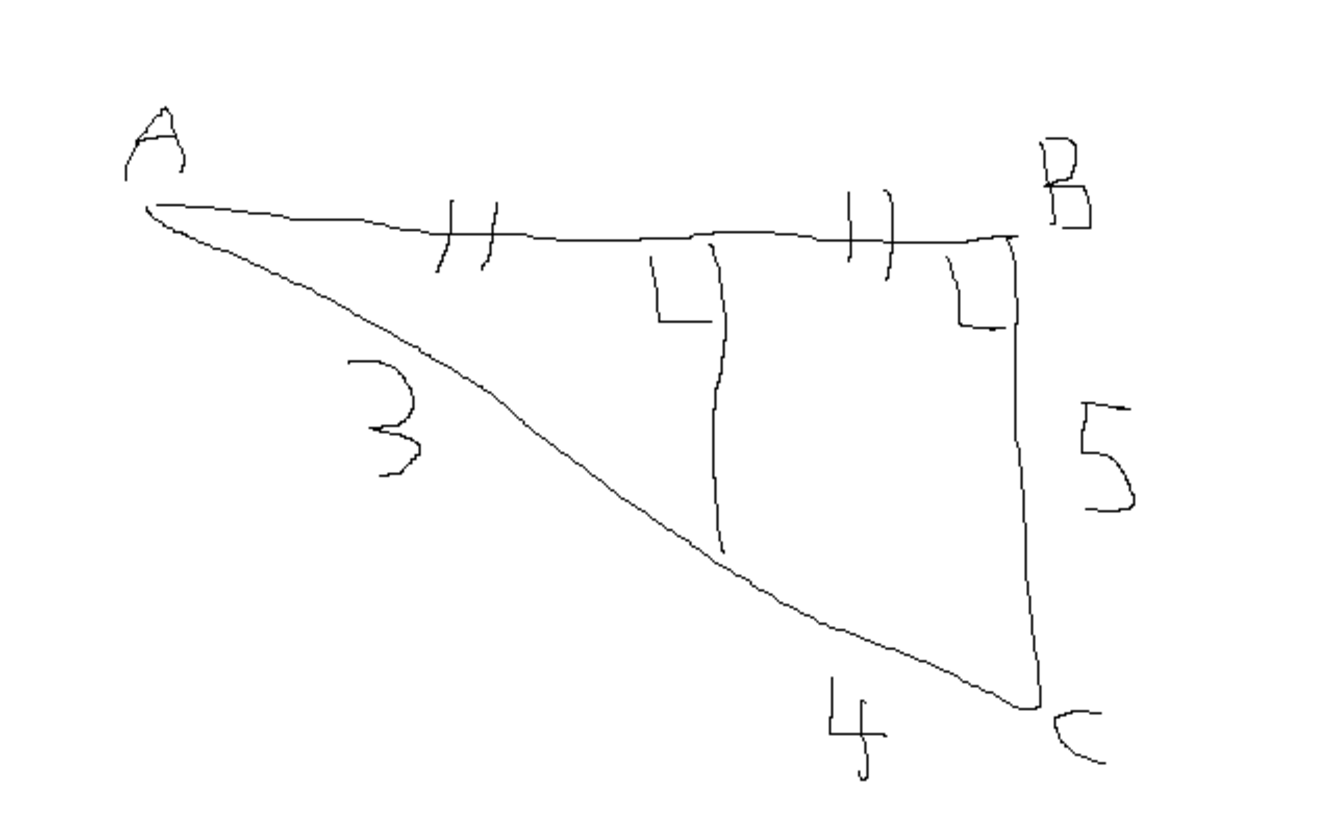
\includegraphics[width=4cm]{faux_triangle.pdf}

    Les mesures sont en centimètres. Est-il possible de tracer en vraie grandeur une figure respectant toutes les conditions ? Si oui le dessiner, sinon, expliquer pourquoi.


\corrref{2smath-0093}
\end{exercice}
